\section{ICP}
\label{ICP}
As an extension to the methods that were discussed in the lectures for the 3D reconstruction we have chosen to implement the Iterative Closest Point (ICP) algorithm using the implementation of \cite{ICP}. It is a algorithm that will minimize the distance between two point clouds. We hoped that this would work on the structure point clouds generated by the structure from motion. It works as follows:

\begin{itemize}
	\item For $N$ iterations, or until converged do the following:
	\begin{itemize}
		\item For every point in the source cloud find the closest point in the reference cloud.
		\item Estimate the combination of rotation and translation using a mean squared error cost function that will best align each source point to its match found in the previous step.
		\item Transform the source points using the obtained transformation.
	\end{itemize}
\end{itemize}

As ICP only works on pairs of images we decided that the best way to merge these is to first do the pairs of images without overlap, so we transformed $im_2$ to match $im_1$ and $im_4$ to match $im_3$ and so on. We then merged the remaining point clouds in the same way.

If this would all go well we could use it to reconstruct the teddy bear from the 3D point clouds. In Figure~\ref{fig:3D} one can see the final results of using ICP on the point clouds generated by the Structure from Motion. It is clear that ICP was not the success that we thought it would be. We have tried different ways of merging, iteratively but they have also not proven to be successful. We think that this is because the algorithm does not take scale into account, only translation and rotation. An algorithm that we could have used that does take scale into account is Procrustes Analysis \cite{procrustes}. However we chose ICP over Procrustes Analysis because we felt that the aim of Procrustes Analysis was to obtain a similar place, rotation and size of the point clouds, which is not exactly what we want.

\begin{figure}[ht]
	\centering
	\subfloat{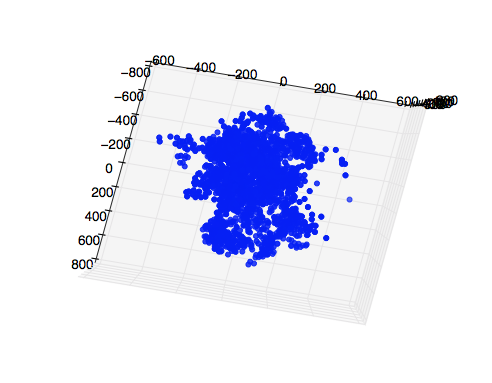
\includegraphics[width=.45\textwidth]{bear_angle1}} \quad
	\subfloat{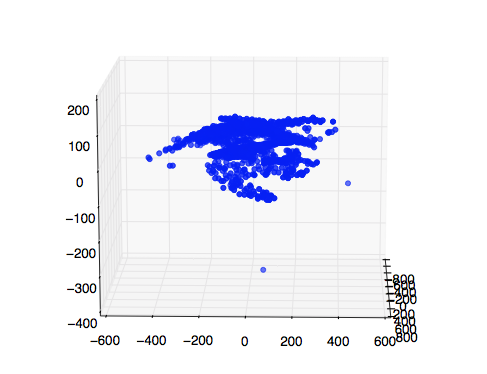
\includegraphics[width=.45\textwidth]{bear_angle2}}
	\caption{The final results of using ICP to merge the point clouds.}
	\label{fig:3D}
\end{figure}
